% SSAC27 Research Paper Competition: abstract submission.
% SSAC rules: fewer than 500 words including title and body; sections Introduction,
% Methods, Results, Conclusion; up to two tables or figures combined.
% No official abstract template is published, so this uses a plain article layout.
% Upload fig1_effect_by_distance.png next to this file on Overleaf. Compile with pdfLaTeX.
\documentclass[11pt]{article}
\usepackage[letterpaper,margin=1in]{geometry}
\usepackage[T1]{fontenc}
\usepackage[utf8]{inputenc}
\usepackage{newtxtext,newtxmath}
\usepackage{graphicx}
\usepackage{float}
\usepackage[font=small,labelfont=bf]{caption}
\usepackage{titlesec}
\usepackage[hidelinks]{hyperref}

\titleformat{\section}{\normalfont\large\bfseries}{}{0pt}{}
\titlespacing*{\section}{0pt}{1.2ex}{0.5ex}
\setlength{\parskip}{0.6ex}
\setlength{\parindent}{0pt}
\pagestyle{plain}

% SSAC: "Final reviews will occur without knowledge of the names of the authors."
% Set \blindtrue to hide the author block for an anonymised PDF.
\newif\ifblind
\blindfalse

\title{\vspace{-1.5cm}\textbf{Shoot or Keep the Ball? A Held-Out Causal Audit of Shot Selection with Public Data}}
\ifblind
  \author{}
\else
  \author{%
    Author One \\ {\small Institution} \\ {\small\texttt{email}} \and
    Author Two \\ {\small Institution} \\ {\small\texttt{email}}%
  }
\fi
\date{}

\begin{document}
\maketitle
\vspace{-1.2cm}

\section*{Introduction}
Every attack in soccer forces a choice: shoot now, or keep the ball by passing, carrying or
dribbling. Comparing these alternatives is hard because players shoot when chances already
look good. Recent tracking-data models recommend when to shoot, without identified causal
effects (Verronneau et al., MLSA 2026). We ask: when players shot, did it pay off compared
with what they would typically have done instead?


\section*{Methods}
We use StatsBomb open event data with 360 freeze-frames (player positions). Decisions are
live-play actions in the attacking third with the ball's 3~m surroundings fully visible.
Each shot is compared with keeping the ball the way players in the same situation actually
did, through the observed mix of passes, carries and dribbles. We compare only where both
choices were realistic (94.9\% of eligible shots). The outcome is the first goal within 15
seconds ($+$1 scored, $-$1 conceded, 0 otherwise). A doubly robust estimator, cross-fitted
by match, adjusts for geometry, pressure, score, time and recent actions. The analysis was
fixed on Euro 2020 and 2024 (102 matches), then run once on World Cup 2022 (64 matches).


\section*{Results}
Before weighting, shots and other decisions sit 2.2 standard deviations apart in distance to
goal; after, every adjusted feature is within 0.08. In the World Cup (1,228 shots; 20,532
other decisions), the net scoring rate was 10.7\% after shots, against an estimated 7.7\%
had the same players kept the ball: a gain of 3.1 percentage points (95\% CI 0.7 to 5.5,
clustered by match), about a third of the raw gap of 8.4 (Figure~\ref{fig:rawadj}).

It is robust: alternative outcome models and estimators give 2.8 to 3.4; measuring goals
over 5, 10 or 30 seconds gives 3.2 to 3.9; leaving out any one match or team gives 2.3 to
4.1. Randomly reassigned shots show no effect, and in 400 simulations with known effects,
intervals contained the truth 93\% of the time.

In both tournaments the gain is concentrated in shots inside 18~m
(Figure~\ref{fig:distance}; World Cup $+$5.9, 2.2 to 9.7), not beyond ($-$1.3); these
prespecified subgroups each narrowly miss one balance threshold, and their difference was
not tested.

The limits are measured. The Euro estimate points the same way but is uncertain (1.8; $-$0.2
to 3.8). Clustering by opponent widens the interval to include zero ($-$0.3 to 6.4), and
hidden factors shifting shooting odds 1.35-fold would bring its lower bound to zero.


\section*{Conclusion}
Public event data can answer what expected goals cannot: what shooting added over the
realistic alternative. Under stated assumptions, in a tournament held out from every design
decision, players' shots added about three percentage points of net scoring rate, robust
across estimators, horizons, matches and teams, with the limits quantified. The result is a
rerunnable public audit for testing shot-selection claims, including those of recommendation
models.

\begin{figure}[H]
  \centering
  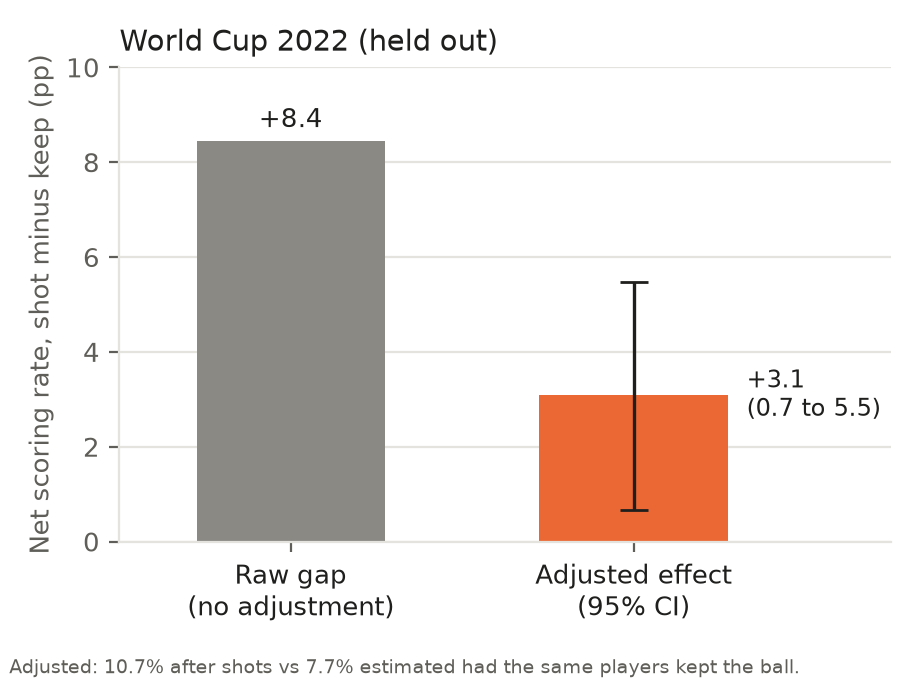
\includegraphics[width=0.62\linewidth]{fig5_estimate_and_uncertainty.png}
  \caption{Raw vs adjusted effect, World Cup.}
  \label{fig:rawadj}
\end{figure}

\begin{figure}[H]
  \centering
  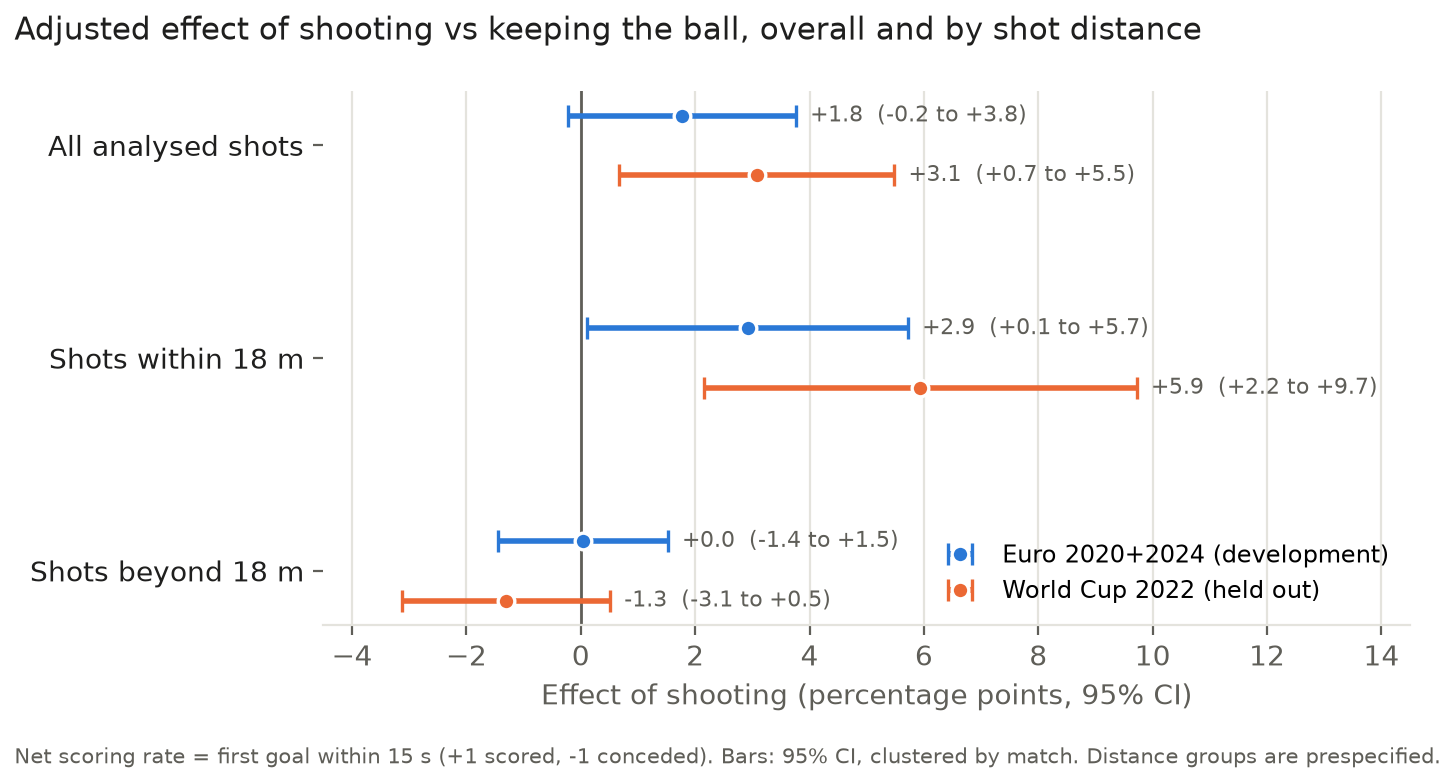
\includegraphics[width=\linewidth]{fig1_effect_by_distance.png}
  \caption{Adjusted effect by shot distance.}
  \label{fig:distance}
\end{figure}

\end{document}
